% do stuff for systems of differential equations, matrix exponential and stuff

    \section*{Introduction}
        Often times a single number is not adequate for describing a quantity.  Take for example, position and velocity.  In order to describe the position or velocity of a particle, we need to know where in space the particle lies as well as the direction in space the particle travels along with its speed.  This takes three numbers to describe (since we move in a 3-dimensional space). Compare this to temperature.  At any given point in space, we can describe the temperature with a single number. 
        
        The quantity being described above is called a vector.  Formally, a vector is an object that can be scaled and added to other vectors of the same type. This allows one to think of more abstract objects as vectors. For example, we can think of solutions to Schr\"odinger's equation (which are functions) as being vectors in their own type of vector space.
        
        Another way to think of a vector is as a list of numbers. Computer scientists tend to think this way, and we will adopt this point of view for this part of the class.  The vector space for solutions to differential equations behaves slightly differently.  Here, we cover only finite dimensional spaces which is the key difference between the point of view that a vector is a list of numbers versus the view that vectors satisfy some rules of addition and scaling.
        
        The study of vectors, the spaces they reside in, and how they transform falls under the name \boldgreen{linear algebra}. Whether you have been told or not, linear algebra has dictated much of the mathematics you have learned.  This is due to the fact that computations in linear algebra are generally very tractable.  We saw examples of linear differential equations previously.  One then saw approximation of functions via Taylor series.  Fundamentally, linear algebra underlies both of these subjects. Together, one could turn any non-linear differential equation, into a linear one in which we could solve using a power series.
        
        Linear algebra itself has a huge amount of application.  It is widely used in computation and graphics.  One also sees its use in optimization or machine learning.  Quantum mechanics is deeply rooted in linear algebra as well. However, aside from spin systems, quantum systems have an underlying vector space which is infinite dimensional!  For now, we will stick with the finite dimensional case.
        
        \section{Vector Spaces}
        
        Vector spaces are the worlds in which vectors reside.  Of course, before we talk about the spaces these objects live in, we should describe the objects as well. The two important quantities in vectors are the vectors themselves and the numbers that scale them.  We'll define these immediately.
        
        \begin{df}{Scalar}{scalar}
        A \boldgreen{scalar} \index{scalar} is an element of a \emph{field} $\mathbb{F}$.  Typically, we take scalars to be numbers $x\in \R$ or $z\in \C$. In other words, we choose our field $\mathbb{F}$ to be equal to $\R$ or $\C$.
        \end{df}
        
        I won't define what a field is here, since we don't need that definition at all.  We will always be working with scalars that are real or complex numbers and we will avoid other scalars.  That isn't to say they aren't important, we just don't need them for our applications.
        
        \begin{exercise}
            If you are interested, look up what a field is and show that $\R$ and $\C$ are fields.
        \end{exercise}
        
        With that in place, we can describe vectors and their associated spaces in a single definition.  
        
        \begin{df}{Vectors and Vector Spaces}{vector}
            A \boldgreen{vector space} $V$ over a field $\mathbb{F}$ is a set of elements we call \boldgreen{vectors} that satisfy the following properties. Take vectors $\vecu,\vecv,\vecw \in V$ and scalars $\alpha, \beta \in \mathbb{F}$. Then, we require that $\alpha\vecv + \beta\vecu \in V$ and 
            \begin{enumerate}[(i)]
                \item (Commutivity of vector addition)
                \[
                \vecu+\vecv=\vecv+\vecu
                \]
                \item (Associativity of vector addition)
                \[
                \vecu+(\vecv+\vecw)=(\vecu+\vecv)+\vecw;
                \]
                \item (Neutral element) There exists $\zerovec$ such that
                \[
                \zerovec+\vecv=\vecv;
                \]
                \item (Inverse element) For each $\vecv$ there exists $-\vecv$ such that
                \[
                \vecv+(-\vecv)=\zerovec;
                \]                
                \item (Assosciativity of scalar multiplication) We have
                \[
                \alpha(\beta \vecv)=(\alpha \beta)\vecv;
                \]
                \item (Distribution over vector addition) we have
                \[
                \alpha(\vecu+\vecv)=\alpha \vecu + \alpha \vecv;
                \]
                \item (Distribution over field addition) we have
                \[
                (\alpha+\beta)\vecv = \alpha \vecv + \beta \vecv;
                \]
                \item (Unit element) There exists $1\in \mathbb{F}$ such that
                \[
                1\vecv = \vecv.
                \]
            \end{enumerate}
        \end{df}
        
        One can try to remember the above rules by the acronym $CANI ADDU$.  The first four have to do with the addition operation and the last four have to do with the scalar multiplication.
        
        \begin{remark}
            It is a common practice to denote vectors as bold symbols or with arrows over the top.  Here we use both to make them more distinguished.  For example, above we used $\vecu$ and $\vecv$ to denote a vector.  We also tend to use Greek letters to denote scalars.  Above we used $\alpha$ and $\beta$ for scalar elements.
        \end{remark}
        
        Now, the above definition is very abstract and we will continually revisit it. But, for now, we should think of vectors as being real geometrical and physical quantities.   In short, a vector space allows for addition of elements we call vectors and scaling of vectors by numbers we calls scalars. 
        
        The geometrical picture of a vector is often most helpful.  Typically, we represent a vector $\vecv$ as an arrow starting with a tail at the origin 0, and head at the desired point. We often do not distinguish a vector $\vecv$ from the point at which the tip lies.  Let us consider the following.
        
        \begin{ex}{Vectors in the Plane $\R^2$}{planar_vectors}
            We denote the 2-dimensional real plane by the symbol $\R^2$. This is a vector space of 2-dimensions with underlying field the real numbers $\R$. The naming convention follows that of the 1-dimensional real line $\R$.  The plane simply has two copies of the real line that provide coordinates for points in the plane.
            
            When specifying a point in the plane, we must provide two coordinates. We saw this previously with complex numbers when we had to provide both a real and imaginary part.  Here in the plane, we tend to think of providing an $x$-value and a $y$-value in a pair $(x,y)$.  
            
            For example, consider the point $(1,2)\in \R^2$.  Then, we can imagine a vector $\vecv$ with tip at $(1,2)$ and tail at the origin $(0,0)$ being given by
            \[
            \vecv = \begin{pmatrix} 1 \\ 2 \end{pmatrix}.
            \]
        \begin{center}
        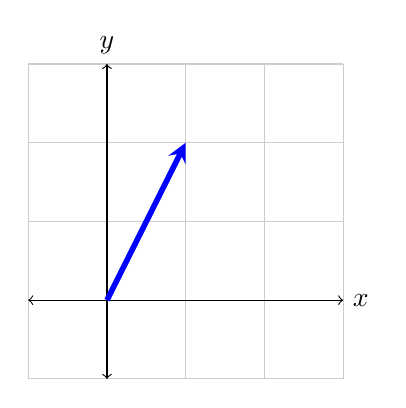
\begin{tikzpicture}
        \draw[thin,gray!40] (-1,-1) grid (3,3);
        \draw[<->] (-1,0)--(3,0) node[right]{$x$};
        \draw[<->] (0,-1)--(0,3) node[above]{$y$};
        \draw[line width=2pt,blue,-stealth](0,0)--(1,2) node[anchor=south west]{$\vecv$};
        \end{tikzpicture}
        \end{center}
        
            Notice that we are barely distinguishing a vector $\vecv$ from the point at which it lies at.  We simply are providing a different notation for it, in some sense.
        \end{ex}
        

        
        \begin{ex}{Positions in 3-Dimensional Space}{position_3dspace}
        The next step up from planar vectors would be vectors in space. Specifically, when we say space we mean a 3-dimensional space $\R^3$.  This is the space we live in in our day to day lives. If you are standing in place, you can measure the position of an object and note that it lies at the point $p=(3,5,4)$ relative to yourself $\zerovec$. This position can described  with a vector and the vector has a bit more structure than just points in space.  This vector begins at your body, and ends at the object. Moreover, it provides you the oriented line segment exiting your eyes and ending at the object. Similarly to the previous example, we would write
        \[
        \vecv = \begin{pmatrix} 3 \\ 5 \\ 4 \end{pmatrix}.
        \]
        We refer to this notation for a vector as a \boldgreen{column vector}. Here, the first entry provides the $x$-coordinate, the second provides the $y$-coordinate, and the third provides the $z$-coordinate. We can picture this vector as follows.
        
        
\begin{center}
\tdplotsetmaincoords{60}{120} 
\begin{tikzpicture} [scale=3, tdplot_main_coords, axis/.style={->,black,thick}, 
vector/.style={-stealth,blue,very thick}, 
vector guide/.style={dashed,red,thick}]

%standard tikz coordinate definition using x, y, z coords
\coordinate (O) at (0,0,0);

%tikz-3dplot coordinate definition using x, y, z coords

\pgfmathsetmacro{\ax}{0.6}
\pgfmathsetmacro{\ay}{1}
\pgfmathsetmacro{\az}{0.8}

\coordinate (P) at (\ax,\ay,\az);

%draw axes
\draw[axis] (0,0,0) -- (1,0,0) node[anchor=north east]{$x$};
\draw[axis] (0,0,0) -- (0,1,0) node[anchor=north west]{$y$};
\draw[axis] (0,0,0) -- (0,0,1) node[anchor=south]{$z$};

%draw a vector from O to P
\draw[vector] (O) -- (P) node[anchor=south east] at (.3,.5,.4){$\vecv$};

%draw guide lines to components
\draw[vector guide]         (O) -- (\ax,\ay,0);
\draw[vector guide] (\ax,\ay,0) -- (P);
\draw[vector guide]         (P) -- (0,0,\az);
\draw[vector guide] (\ax,\ay,0) -- (0,\ay,0);
\draw[vector guide] (\ax,\ay,0) -- (0,\ay,0);
\draw[vector guide] (\ax,\ay,0) -- (\ax,0,0);
\node[tdplot_main_coords,anchor=east]
at (\ax,0,0){};
\node[tdplot_main_coords,anchor=west]
at (0,\ay,0){};
\node[tdplot_main_coords,anchor=south]
at (0,0,\az){};
\node[tdplot_main_coords, anchor=south east] at (0,0,0){$\zerovec$};
\node[tdplot_main_coords, anchor=west] at (\ax,\ay,\az){$p$};
\end{tikzpicture}
\end{center}

        If $p$ moves over time, then our vector $\vecv$ changes over time as well. We'll often denote this $\vecv(t)$.  It's possible the position of an object changes due to interactions with the environment or other objects.  All to come later.
        \end{ex}
        
        Great, we have some objects, but what can we do with them?  As it turns out, we can do quite a bit.  For the most part, anything we could do with numbers, we can do with vectors.  However, we have to be comfortable looking at things in new ways.
        
        \section{Vector Algebra}
        
        Described in the vector space definition is an operation called \boldgreen{vector addition}.  Given two vectors $\vecu$ and $\vecv$, we can create a new vector
        \[
        \vecw = \vecu + \vecv
        \]
        We then required that addition is a commutative operation and so we also have that
        \[
        \vecw = \vecv+\vecu
        \]
        Pictorially, what do we do when we add vectors? We take $\vecu$ and attach the tail of $\vecv$ to the head $\vecu$. 
        
        \begin{center}
        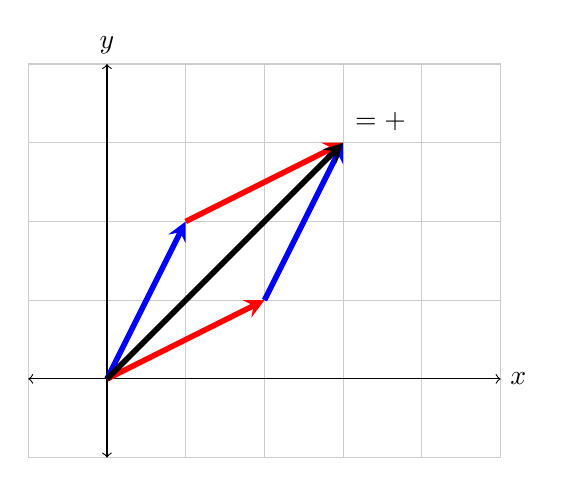
\begin{tikzpicture}
        \draw[thin,gray!40] (-1,-1) grid (5,4);
        \draw[<->] (-1,0)--(5,0) node[right]{$x$};
        \draw[<->] (0,-1)--(0,4) node[above]{$y$};
        \draw[line width=2pt,blue,-stealth](0,0)--(1,2) node[anchor=east] at (.5,1){$\vecu$};
        \draw[line width=2pt, red, -stealth](0,0)--(2,1) node[anchor=north] at (1,.5){$\vecv$};
        \draw[line width=2pt, red, -stealth](1,2)--(3,3) node[anchor=south] at (2,2.5){$\vecv$};
        \draw[line width=2pt, blue, -stealth](2,1)--(3,3) node[anchor=west] at (2.5,2){$\vecu$};
        \draw[line width=2pt, black, -stealth](0,0)--(3,3) node[anchor=south west]{$\vecw=\vecu+\vecv$};
        \end{tikzpicture}
        \end{center}
        
        From this diagram, you can see why the operation is commutative.  Both paths, $\vecu+\vecv$ and $\vecv+\vecu$, lead to the same $\vecw$.
        
        As always, repeated addition gives us a form of multiplication. What will this mean here? 
        
        \begin{exercise}
        Draw a 2-dimensional coordinate system ($x$ and $y$ axes), and draw some vector $\vecv$.  Using vector addition, what does $\vecv+\vecv=2\vecv$ look like? Given this, what do you think $\frac{1}{2}\vecv$ will look like? 
        \end{exercise}
        
        When dealing with a vector, we are allowed to scale the length of the arrow.  As in the definition for a vector space, we call this \boldgreen{scalar multiplication}. Since the vector $2\vecv$ has twice the length of $\vecv$, we would expect $\frac{1}{2} \vecv$ to have half the length of $\vecv$.  All of these vectors point in the same direction though.  We have merely scaled their lengths.
        
        \begin{question}
        What happens if we take $-\vecv$ (i.e., $-1\cdot \vecv$)? \emph{Hint: Consider what happens for numbers on a number line when multiplied by $-1$.} 
        \end{question}
        
        \begin{answer}
        It flips the direction of the vector.
        \end{answer}
        
        We can take a look at all of this. 
        
        \begin{center}
        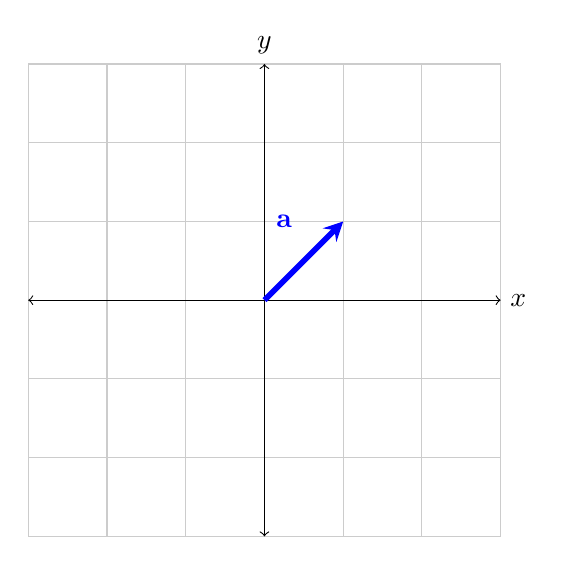
\begin{tikzpicture}
        \draw[thin,gray!40] (-3,-3) grid (3,3);
        \draw[<->] (-3,0)--(3,0) node[right]{$x$};
        \draw[<->] (0,-3)--(0,3) node[above]{$y$};
        \draw[line width=2pt,blue,-stealth](0,0)--(1,1) node[anchor=east] at (.5,1){$\mathbf{a}$};
        \end{tikzpicture}
        \qquad
        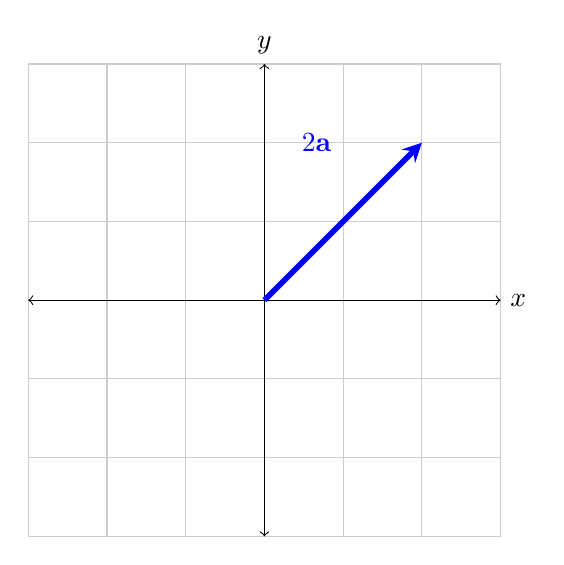
\begin{tikzpicture}
        \draw[thin,gray!40] (-3,-3) grid (3,3);
        \draw[<->] (-3,0)--(3,0) node[right]{$x$};
        \draw[<->] (0,-3)--(0,3) node[above]{$y$};
        \draw[line width=2pt,blue,-stealth](0,0)--(2,2) node[anchor=east] at (1,2){$2\mathbf{a}$};
        \end{tikzpicture}
        
        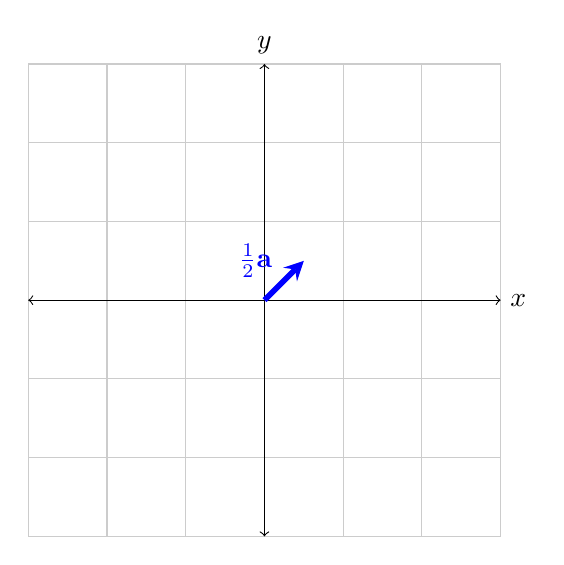
\begin{tikzpicture}
        \draw[thin,gray!40] (-3,-3) grid (3,3);
        \draw[<->] (-3,0)--(3,0) node[right]{$x$};
        \draw[<->] (0,-3)--(0,3) node[above]{$y$};
        \draw[line width=2pt,blue,-stealth](0,0)--(.5,.5) node[anchor=east] at (.25,.5){$\frac{1}{2}\mathbf{a}$};
        \end{tikzpicture}
        \qquad
        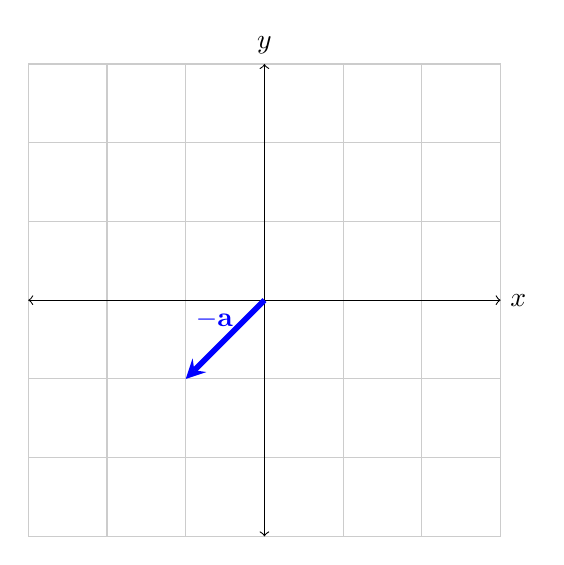
\begin{tikzpicture}
        \draw[thin,gray!40] (-3,-3) grid (3,3);
        \draw[<->] (-3,0)--(3,0) node[right]{$x$};
        \draw[<->] (0,-3)--(0,3) node[above]{$y$};
        \draw[line width=2pt,blue,-stealth](0,0)--(-1,-1) node[anchor=east] at (-.25,-.25){$-\mathbf{a}$};
        \end{tikzpicture}
        \end{center}
        
        In the definition for a vector space, we also required that there exists an inverse element for the vector $\vecv$. That is, we wanted to find a vector $\vecu$ so that $\vecv+\vecu=\zerovec$.  Notice that if we take $\vecu=-\vecv$, then we have $\vecv+(-\vecv)=\zerovec$ using the geometrical notion of vector addition shown above.  Thus, additive inverses of vectors are just vectors of the same length pointing in the opposite direction.  This also gives us a notion of subtracting vectors.
        
        \begin{question}
        Given two arbitrary vectors $\vecu$ and $\vecv$, how can we define $\vecu-\vecv$?  
        \end{question}
        
        \begin{answer}
        As we did above for the inverse case. We write $\vecu+(-\vecv)$ and use the rules for vector addition and scalar multiplication together.
        \end{answer}
        
        \begin{exercise}
        Draw two different vectors $\vecu$ and $\vecv$ and draw the following:
        \begin{itemize}
            \item $\vecu+\vecv$,
            \item $\vecu-\vecv$,
            \item $\vecv-\vecu$.
        \end{itemize}
        \end{exercise}
        
        Now see the picture below.
        
        \begin{center}
        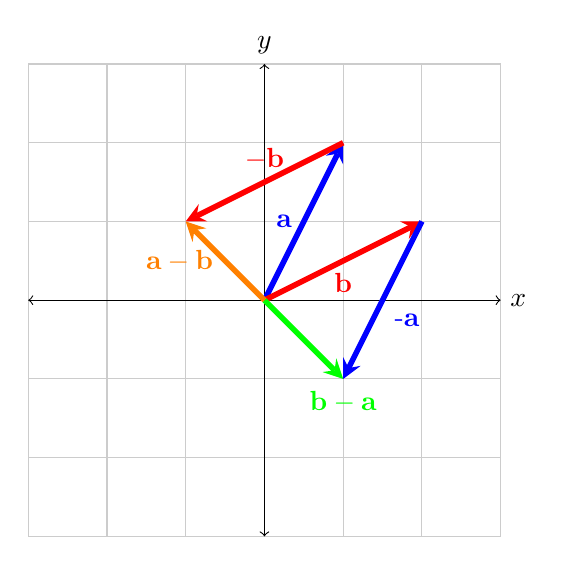
\begin{tikzpicture}
        \draw[thin,gray!40] (-3,-3) grid (3,3);
        \draw[<->] (-3,0)--(3,0) node[right]{$x$};
        \draw[<->] (0,-3)--(0,3) node[above]{$y$};
        \draw[line width=2pt,blue,-stealth](0,0)--(1,2) node[anchor=east] at (.5,1){$\mathbf{a}$};
        \draw[line width=2pt, red, -stealth](0,0)--(2,1) node[anchor=north] at (1,.5){$\mathbf{b}$};
        \draw[line width=2pt, red, -stealth](1,2)--(-1,1) node[anchor=south] at (0,1.5){$-\mathbf{b}$};
        \draw[line width=2pt, blue, -stealth](2,1)--(1,-1) node[anchor=west] at (1.5,-.25){-$\mathbf{a}$};
        \draw[line width=2pt, green, -stealth](0,0)--(1,-1) node[anchor=north]{$\mathbf{b}-\mathbf{a}$};
        \draw[line width=2pt, orange, -stealth](0,0)--(-1,1) node[anchor=east] at (-.5,.5){$\mathbf{a}-\mathbf{b}$};
        \end{tikzpicture}
        \end{center}
        
        \subsection{Linear Combinations}
        
        The most important notion in linear algebra is that of a \boldgreen{linear combination} or \boldgreen{superposition}.  Each and every axiom we required in the definition is put there in order to make sense of linear combinations.  Given two vectors $\vecu,\vecv\in V$ and two scalars $\alpha, \beta \in \mathbb{F}$ from the underlying field $\mathbb{F}$, we call 
        \[
        \alpha \vecu + \beta \vecv
        \]
        a linear combination.  
        
        The requirements in our definition allow us to geometrically interpret scalar multiplication and vector addition as we do, and we can string both of these concepts together in one linear combination.  Vector addition itself is a linear combination where the scalars are chosen to both be one, and scalar multiplication could just be a linear combination with one of the vectors the zero vector.
        
        Linear combinations then allow us to understand how to break up vectors and better use coordinates to describe them.  Similar to coordinates on Earth (i.e., latitude and longitude) we need numbers to describe a vector. But, we also need to know what these numbers are specifying.  We know what latitude and longitude describe on Earth, but these are not the only choice in coordinates we could use!
        
        \section{Vector Components}
        The previous work has still been fairly abstract and has left us without a way to explicitly compute quantities! To work with vectors more effectively, it's necessary to break them down into \boldgreen{components}. We can think of components as coming from coordinates on the vector space. Let us consider the following.
        
        \begin{ex}{Components of a Vector}{vector_components}
        Let us fix an arbitrary vector $\vecv$ in $\R^2$ (i.e., the $xy$-plane).  
        \begin{center}
        \begin{tikzpicture}[vector guide/.style={dashed,red,thick}]
        \draw[<->] (-1,0)--(5,0) node[right]{$x$};
        \draw[<->] (0,-1)--(0,5) node[above]{$y$};
        \draw[line width=2pt,blue,-stealth](0,0)--(4,4) node[anchor=east] at (2,2.5){$\vecv$};
        \draw[vector guide] (4,0) -- (4,4);
        \draw[vector guide] (0,0) -- (4,0);
        \node[anchor=north] at (2,0){$v_x$};
        \node[anchor=west] at (4,2){$v_y$};
        \end{tikzpicture}
        \end{center}
        We can break down this vector into the portions that are in the $x$-direction and $y$-direction.  We say that the component of the vector in the $x$-direction is $v_x$ and the component of the vector in the $y$-direction is $v_y$.  Using the Pythagorean theorem, it follows that the length of the vector is $\|\vecv\|=\sqrt{v_x^2+v_y^2}$. This is exactly how we defined the modulus of a complex number $\|z\|$.
        
        Hence, we would write
        \[
        \vecv=\begin{pmatrix} v_x \\ v_y \end{pmatrix}.
        \]
        \end{ex} 
        
        In the previous two examples we represented vectors by ordered lists of numbers.  This notation is more than adequate, but we do often see vectors presented a different way. When we think of vectors, we tend to think of coordinates presented in the ordered list.  However, we will sometimes wish to change coordinates and so we must consider the other form of notation. These coordinates would then give us different components for a vector.  We will eventually see this.
        
        \section{Vector Algebra with Components}
        Let us work with vectors in space $\R^3$.  These vectors each have three components, so it suffices to specify $\vecv$ as 
        \[
        \vecv = \begin{pmatrix} v_x \\ v_y \\ v_z \end{pmatrix}.
        \]
        One can then also specify the length $\|\vecv\|$ of $\vecv$ by writing
        \[
        \|\vecv\| = \sqrt{ v_x^2 + v_y^2 + v_z^2},
        \]
        which is much like the Pythagorean theorem. If a vector $\unitvec$ has length one, that is, if $\|\unitvec\|=1$, then we say that $\unitvec$ is a \boldgreen{unit vector}. One may also say that $\unitvec$ is a \boldgreen{normalized} vector. We also tend to place hats on unit vectors as opposed to arrows to denote the unit length.
        
        When we write these coordinates for a vector, we are really saying that $\vecv$ points an amount $v_x$ in the $x$-direction, $v_y$ in the $y$-direction, and $v_z$ in the $z$-direction.  So, if we consider unit vectors that point in these different directions, then we can  write $\vecv$ as a linear combination of these vectors.  So, we set
        \[
        \xhat = \begin{pmatrix} 1 \\ 0 \\ 0 \end{pmatrix} \qquad \yhat = \begin{pmatrix} 0 \\ 1 \\ 0 \end{pmatrix} \qquad \zhat = \begin{pmatrix} 0 \\ 0 \\ 1 \end{pmatrix}.
        \]
        We call the above vectors the \boldgreen{unit basis vectors} since they are of  length one and we can write any vector in $\R^3$ as a linear combination of the three of them.  That is, we can write 
        \[
        \vecv = v_x \xhat + v_y \yhat + v_z \zhat.
        \]
        

        Now, we want to be able to understand vector algebra in these components. Let 
        \[
        \vecu = u_x \xhat + u_y \yhat + u_z \zhat \qquad \textrm{and} \qquad \vecv = v_x \xhat + v_y \yhat + v_z \zhat,
        \]
        then we can note the following:
        
        \begin{itemize}
            \item \textbf{Equality:} Vectors are equal when their components are equal,
            \[
            \vecu=\vecv ~~ \textrm{if} ~~ u_x=v_x, ~~ u_y=v_y ~~ \textrm{and} ~~ u_z=v_z.
            \]
            \item \textbf{Addition:} The sum $\vecu + \vecv$ is done by adding components together,
            \[
            \vecu+\vecv=(u_x+v_x)\xhat + (u_y + v_y)\yhat + (u_z + v_z)\zhat.
            \]
            \item \textbf{Scalar Multiplication:} The product $\alpha \vecv$ is obtained by multiplying each component of $\vecv$ by $\alpha$,
            \[
            \alpha \vecv = (\alpha v_x) \xhat + (\alpha v_y)\yhat + (\alpha v_z)\zhat.
            \]
        \end{itemize}
        
        \begin{ex}{Vector Algebra in Space}{vect_alg_space}
            Consider the vectors
            \[
            \vecu = \xhat + \yhat + \zhat = \begin{pmatrix} 1 \\ 1 \\ 1\end{pmatrix} \qquad \vecv = 2\xhat + \yhat = \begin{pmatrix} 2 \\ 1 \\ 0 \end{pmatrix} \qquad \vecw = \xhat + \zhat = \begin{pmatrix} 1 \\ 0 \\ 1 \end{pmatrix}.
            \]
            Then we can compute 
            \[
            \vecu+\vecv = (\xhat+\yhat+\zhat)+(2\xhat + \yhat) = 3\xhat + 2\yhat + \zhat.
            \]
            Or, we can add the column vectors
            \[
            \vecu+\vecv = \begin{pmatrix} 1 \\ 1 \\ 1 \end{pmatrix} + \begin{pmatrix} 2 \\ 1 \\ 0 \end{pmatrix} = \begin{pmatrix} 3 \\ 2 \\ 1 \end{pmatrix}.
            \]
            Of course, we could also sum all three vectors and find
            \[
            \vecu+\vecv+\vecw = 4\xhat + 2\yhat + 2 \zhat = \begin{pmatrix} 4 \\ 2 \\ 2 \end{pmatrix}.
            \]
            We can also scale the vectors. Take for example
            \[
            5 \vecu = 5\xhat + 5\yhat + 5\zhat = \begin{pmatrix} 5 \\ 5 \\ 5 \end{pmatrix}
            \]
            or
            \[
            - \vecv = -2\xhat -\yhat = \begin{pmatrix} -2 \\ -1 \\ 0 \end{pmatrix}.
            \]
            Then, we could consider a linear combination of the vectors like
            \begin{align*}
                5\vecu - \vecv + 2\vecw &= (5\xhat + 5\yhat + 5\zhat) + (-2\xhat -\yhat) + (2\xhat +2\zhat)\\
                &= 5\xhat + 4\yhat +7\zhat\\
                &= \begin{pmatrix} 5 \\ 4 \\ 7 \end{pmatrix}.
            \end{align*}
        \end{ex}
        
        \begin{exercise}
            Draw the picture for the subtraction $\vecu-\vecv$.
        \end{exercise}
        
        \begin{exercise}
        Given $\vecu=(2,3,1)$, $\vecv=(1,-2,0)$, and $\vecw=(5,2,-1)$, find 
        \begin{enumerate}[(a)]
            \item $\boldsymbol{\vec{d}}=2\vecu+3\vecv-\vecw$,
            \item $\|\boldsymbol{\vec{d}}\|$ (the length of $\boldsymbol{\vec{d}}$),
            \item Let $\alpha$ be a scalar.  Does it make sense to consider $\boldsymbol{\vec{r}}=\vecu+\alpha$? Why or why not?
        \end{enumerate}
        \end{exercise}
        
        Given a vector space $V$, we want to find a list of vectors that, by taking a linear combination of said vectors, can form any vector in the vector space $V$.  We call this set of vectors a \boldgreen{basis}. Given a set of vectors $\{\vecv_1,\vecv_2,\dots,\vecv_n\}$, we say that the \boldgreen{span} of the vectors is the set of all vectors that can be written as linear combinations of the vectors in the set.  Specifically, we are looking for all vectors $\vecu$ so that
        \[
        \vecu = \alpha_1 \vecv_1 + \alpha_2 \vecv_2 +\cdots + \alpha_n \vecv_n.
        \]
        Then we can define the span (which is a set) to be
        \[
        \Span(\{\vecv_1,\vecv_2,\dots,\vecv_n\}) = \{\alpha_1 \vecv_1 + \alpha_2 \vecv_2 +\cdots + \alpha_n \vecv_n ~|~ \alpha_i \in \mathbb{F}\}.
        \]
        
        Take for example vectors in the real plane $\R^2$.  We have that the unit basis vectors $\xhat$ and $\yhat$ form a basis for $\R^2$ since any vector $\vecv$ can be written as a linear combination as 
        \[
        \vecv = v_x \xhat + v_y\yhat.
        \]
        Similarly, a vector $\vecu$ in space $\R^3$ can be written as a linear combination of the unit basis vectors $\xhat$, $\yhat$, and $\zhat$ as
        \[
        \vecu = u_x \xhat + u_y \yhat + u_z \zhat.
        \]
        Hence the unit basis vectors for $\R^3$ are also a basis.  One shouldn't have been surprised based on the name we chose!
        
        We can visualize these basis vectors in the plane and make sense of the combinations above. Let us take the vector $\vecv = 2\xhat + 3\yhat$, then we have:
        \begin{center}
        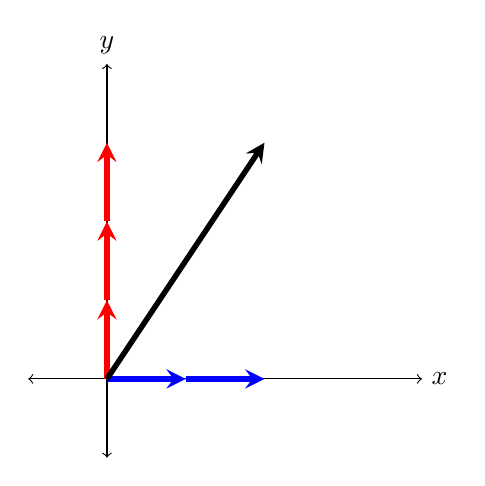
\begin{tikzpicture}[vector guide/.style={dashed,red,thick}]
        \draw[<->] (-1,0)--(4,0) node[right]{$x$};
        \draw[<->] (0,-1)--(0,4) node[above]{$y$};
        \draw[line width=2pt,blue,-stealth](0,0)--(1,0) node[anchor=north] at (1,0){$\xhat$};
        \draw[line width=2pt,blue,-stealth](1,0)--(2,0) node[anchor=north] at (2,0){$\xhat$};
        \draw[line width=2pt, red,-stealth](0,0)--(0,1) node[anchor=east] at (0,1){$\yhat$};
        \draw[line width=2pt, red,-stealth](0,1)--(0,2) node[anchor=east] at (0,2){$\yhat$};
        \draw[line width=2pt, red,-stealth](0,2)--(0,3) node[anchor=east] at (0,3){$\yhat$};
        \draw[line width=2pt,black,-stealth](0,0)--(2,3) node[anchor=north] at (2,3){$\vecv$};
        \end{tikzpicture}
        \end{center}
        
        \begin{ex}{Another Basis for $\R^3$}{another_basis}
        Consider again the vectors
            \[
            \vecu = \xhat + \yhat + \zhat = \begin{pmatrix} 1 \\ 1 \\ 1\end{pmatrix} \qquad \vecv = 2\xhat + \yhat = \begin{pmatrix} 2 \\ 1 \\ 0 \end{pmatrix} \qquad \vecw = \xhat + \zhat = \begin{pmatrix} 1 \\ 0 \\ 1 \end{pmatrix},
            \]
            then these vectors form a basis for $\R^3$. 
            \begin{question}
            How do we show that this is a basis?
            \end{question}
            \begin{answer}
            We must show that any vector $\vecr \in \R^3$ can be written as a linear combination of the three given vectors.
            \end{answer}
            So, let $\vecr = r_x\xhat + r_y\yhat + r_z \zhat$, and we have
            \begin{align*}
                \vecr &= \alpha_1 \vecu + \alpha_2 \vecv + \alpha_3 \vecw\\
                u_x \xhat + u_y \yhat + u_z \zhat &= \alpha_1 (\xhat + \yhat + \zhat) + \alpha_2 (2\xhat + \yhat) + \alpha_3 (\xhat + \zhat)\\
                u_x \xhat + u_y \yhat + u_z \zhat &= (\alpha_1 +2\alpha_2 + \alpha_3)\xhat + (\alpha_1 +\alpha_2)\yhat + (\alpha_1 +\alpha_3)\zhat.
            \end{align*}
            This gives us three equations. One for each component of the vector $\vecu$. Specifically, we have
            \begin{align*}
                u_x &= \alpha_1 + 2\alpha_2 + \alpha_3 \\
                u_y &= \alpha_1 + \alpha_2\\
                u_z &= \alpha_1 + \alpha_3.
            \end{align*}
            The goal is now to determine whether or not this system of equations can be solved in general!
        \end{ex}
        
        Now that we have some structure, it's worth seeing one example of an application for vectors. There are plenty more reasons, but with the tools we already have, this example is not too hard to work with. Plus, it is rather fundamental.
        
        \begin{ex}{Center of Mass}{center_of_mass}
        If we have $n$ point masses each with a mass $m_i$ and position $\boldsymbol{\vec{r}}_i$, then the center of mass can be written
        \[
        \boldsymbol{\vec{R}}_{cm}=\frac{1}{M}(m_1\boldsymbol{\vec{r}}_1+m_2 \boldsymbol{\vec{r}}_2 + \cdots + m_n \boldsymbol{\vec{r}}_n)=\frac{1}{M}\sum_{i=1}^n m_i \boldsymbol{\vec{r}}_i
        \]
        where
        \[
        M=\sum_{i=1}^n m_i
        \]
        is the total mass.
        
        The way to think about this is as averaging the position of these particles but keeping track of how much each weighs.  For example, imagine two masses $m_1$ and $m_2$ in one dimension.  If $\boldsymbol{\vec{r}}_1=1$ and $\boldsymbol{\vec{r}}_2=-1$, then if $m_2>m_1$, the center of mass should be closer to $m_2$ and thus negative.
        \end{ex}
        

        
        The most important vector space for us will be $\R^n$ where $n$ is a positive integer.  $\R^2$ is familiar to us, as it is usually called the $xy$-plane. $\R^3$ is as well, as we usually think of the space surrounding us as being 3-dimensional.
        
        \begin{remark}
        For us, we will always assume that the tail of vectors starts at $\zerovec$ (the origin) unless otherwise stated.  When we get to vector fields, this will be a bit different.
        \end{remark}
        
        \begin{ex}{Examples of Vectors}{examples_of_vecs}
        When the field of scalars are real numbers, we have some example vector spaces. Note, for these, all the scalars $v_x,v_y,v_z,$ or $v_i$ are all real numbers.
        \begin{itemize}
            \item A vector $\vecv \in \R^1=\R$ is just a real number.
            \item A vector $\vecv \in \R^2$ is written as 
            \[
            \vecv = v_x \xhat + v_y \yhat = \begin{pmatrix} v_x \\ v_y \end{pmatrix}.
            \]
            \item A vector $\vecv \in \R^3$ is written as 
            \[
            \vecv = v_x \xhat + v_y \yhat + v_z \zhat = \begin{pmatrix} v_x \\ v_y \\ v_z \end{pmatrix}.
            \]
            \item In general, a vector $\vecv \in \R^n$ is written as
            \[
            \vecv = v_1 \basvec_1 + v_2 \basvec_2 + \cdots + v_n \basvec_n = \begin{pmatrix} v_1 \\ v_2 \\ \vdots \\ v_n \end{pmatrix}.
            \]
            where $\basvec_i$ is the $i$th standard unit basis vector for $\R^n$.
        \end{itemize}
        It is possible that the field of scalars is also the complex numbers, in which case we have analogous vector spaces. Here, we tend to not have special notation for two or three dimensional space and we just put
        \begin{itemize}
            \item A vector $\vecu \in \C^n$ is written as
            \[
            \vecu = u_1 \basvec_1 + u_2 \basvec_2 + \cdots + u_n \basvec_n,
            \]
            where all the $u_i$ are complex numbers.
        \end{itemize}
        \end{ex}
        
        \section{Products of Vectors}
        
        Given two vectors, one would like to make products between them in order to find out how related the two vectors are.  Also, we should be able to decompose any vectors in a vector space into more fundamental components we understand.  We've done this above, but now we would like a way to do this in more generality.
        
        \subsection{The Dot Product}
        \begin{question}
        Given two vectors $\vecu$ and $\vecv$ based at the same point, can we determine the angle $\theta$ between them? 
        \end{question}
        
        \begin{center}
\begin{tikzpicture}
  \draw
    (3,-1) coordinate (a) node[right] {$\vecv$}
    -- (0,0) coordinate (b) node[left] {}
    -- (2,2) coordinate (c) node[above right] {$\vecu$}
    pic["$\theta$", draw=orange, <->, angle eccentricity=1.2, angle radius=1cm]
    {angle=a--b--c};
\end{tikzpicture}
        \end{center}
        
        \begin{answer}
        Yes.  In fact, the way we find this gives us a lot more than just an angle.  It will be a fundamental concept that we will use often.
        \end{answer}
        
        Let's consider the following related question first.  If we have a vector $\vecv$ and a unit vector $\unitvec$, how much of the vector $\vecv$ lies across the vector $\unitvec$? We will denote this quantity by $\vecv\cdot \unitvec$.) The physical way to think about this is to imagine that we are shining a light perpendicularly to $\unitvec$ and we measure the length of the shadow that $\vecv$ would leave on $\unitvec$? Take for example the following illustration.
        
        \begin{center}
        \begin{tikzpicture}[vector guide/.style={dashed,red,thick}]
        \draw[<->] (-1,0)--(4,0) node[right]{$x$};
        \draw[<->] (0,-1)--(0,4) node[above]{$y$};
        \draw[line width=2pt,black,-stealth](0,0)--(2,3) node[anchor=west] at (2,3){$\vecv$};
        \draw[line width=2pt,blue,-stealth](0,0)--(1,0) node[anchor=south west] at (1,0){$\unitvec$};
        \draw[vector guide] (0,-.25) -- (2,-.25) node[anchor=north] at (1,-.25){$\vecv \cdot \unitvec$};
        \end{tikzpicture}
        \end{center}
        
        \noindent Above, one should note that this operation of $\vecv\cdot \unitvec$ is not giving us a new vector, rather it is just providing the length of this shadow being cast.
        
        When the angle is $\theta=0$, then we expect this quantity $\vecv \cdot \unitvec$ to be maximized as the shadow cast by projecting $\vecv$ onto $\unitvec$ will be as long as $\vecv$ is itself. When $\theta=\frac{\pi}{2}$, the quantity will be zero as there will be no shadow cast at all. When $\theta=\pi$, then our quantity would be reversed as to tell us that we would be measuring a shadow pointing the opposite direction of $\unitvec$. This is then the negative of the result that we arrived at when $\theta=0$.  Continuing, if $\theta=\frac{3\pi}{2}$, we would get 0 and lastly if $\theta=2\pi$ this is no different than $\theta=0$.  
        
        What we arrive at with a bit more work is that
        \[
        \vecv\cdot \unitvec=\|\vecv\| \cos \theta.
        \]
        We call this the \boldgreen{dot product} or \boldgreen{inner product} of the vectors $\vecv$ and $\unitvec$. However, we are not required to form this product between a vector and a unit vector. The only difference we see is that the length of the vector we are casting a shadow onto also plays a role in the output of the dot product. Specifically, we have for vectors $\vecv$ and $\vecu$ that the inner product is given by
        \[
        \boxed{\vecu \cdot \vecv = \|\vecu\|\|\vecv\| \cos \theta,}
        \]
        where $\theta$ is again the angle between the two vectors
        
        It turns out that the inner product can be computed in another way.  This fact makes the inner product an indispensable tool. For two vectors given by coordinates $\vecu=(u_x,u_y,u_z)$ and $\vecv=(v_x,v_y,v_z)$ that
        \[
        \boxed{\vecu \cdot \vecv= u_xv_x + u_y v_y + u_z v_z}.
        \]
        Both definitions imply that we have commutivity for this product of vectors. That is,
        \[
        \vecu\cdot \vecv = \vecv \cdot \vecu.
        \]
        They also imply that if we take three vectors, we have
        \[
        (\vecu+\vecv)\cdot \vecw = \vecu \cdot \vecw + \vecv \cdot \vecw.
        \]
        
        \begin{remark}
        If we had vectors $\vecu$ and $\vecv$ that were both elements of $\R^n$, we would compute the dot product just as above. That is, if 
        \[
        \vecu = u_1 \basvec + u_2 \basvec_2 + \cdots + u_n \basvec_n \qquad \vecv = v_1 \basvec_1 + v_2 \basvec_2 + \cdots + v_n \basvec_n,
        \]
        then we have
        \[
        \vecu \cdot \vecv = u_1 v_1 + u_2 v_2 +\cdots + u_n v_n = \sum_{i=1}^n u_i v_i.
        \]
        \end{remark}
        
        The inner product gives us special relationships to vectors. It also gives us a natural notion of direction and lets us compare these directions to one another.  Specifically, the inner product lets us see when two vectors point in two perpendicular directions. 
        
        \begin{df}{Orthogonal}{orthogonal}
        Two vectors $\vecu$ and $\vecv$ are \boldgreen{orthogonal} \index{orthogonal} if
        \[
        \vecu\cdot \vecv=0.
        \]
        Orthogonal and perpendicular are synonymous.
        \end{df}
        
        \begin{ex}{Unit Basis Vectors}{unit_basis_vectors}
            Consider the unit basis vectors in $\R^3$,
            \[
            \xhat = \begin{pmatrix} 1 \\ 0 \\ 0 \end{pmatrix}, \qquad \yhat = \begin{pmatrix} 0 \\ 1 \\ 0 \end{pmatrix}, \qquad \zhat = \begin{pmatrix} 0 \\ 0 \\ 1 \end{pmatrix}.
            \]
            Then each of these unit basis vectors are mutually orthogonal to one another.  Specifically, if we take
            \begin{align*}
            \xhat \cdot \yhat &= 1\cdot 0 + 0 \cdot 1 + 0 \cdot 0 = 0\\
            \xhat \cdot \zhat &= 1\cdot 0 + 0 \cdot 0 + 0 \cdot 1 = 0\\
            \yhat \cdot \zhat &= 0 \cdot 0 + 1\cdot 0 + 0 \cdot 1 = 0.
            \end{align*}
        \end{ex}
        
        \begin{exercise}
        Take two vectors $\vecu=2\xhat + \yhat$ and $\vecv=\xhat + \yhat$.  Compute the dot product in both ways.  That is
        \[
        \vecu\cdot \vecv=u_xv_x + u_y v_y=\|\vecu\|\|\vecv\|\cos \theta.
        \]
        Verify that they give the same answer.
        \end{exercise}
        
        \begin{ex}{Work by Constant Force}{work_constant_force}
        The \boldgreen{work} $W$ done by a constant force $\boldsymbol{\vec{F}}$ on a mass $m$ displaced from position $\vecu=u_x \xhat + u_y \yhat + u_z\zhat $ to $\vecv = v_x \xhat + v_y \yhat + v_z \zhat$ is given by
        \[
        W=\forcevec\cdot \displacement
        \]
        where
        \[
        \displacement=\vecv-\vecu.
        \]
        \end{ex}
        
        \subsubsection{Length of a Vector from the Inner Product}
        The inner product of vectors gives us a natural way to compute the length of a vector.  By the way we defined it, we have that the inner product describes the length of a vector lying along another vector.  So, if we allow both vectors input into the inner product to the same vector, we will find this relates to the length. Take a vector $\vecv \in \R^2$, then we can compute
        \[
        \vecv \cdot \vecv = \|\vecv\|\|\vecv\| \cos \theta,
        \]
        but the angle between the vectors is zero and hence
        \[
        \boxed{\vecv\cdot \vecv = \|\vecv\|^2}.
        \]
        Using the other means of computing the dot product, we have
        \[
        \boxed{\vecv \cdot \vecv = \|\vecv\|^2 = v_x^2 + v_y^2}
        \]
        which is just the Pythagorean theorem!  This of course generalizes to 3-dimensions and higher.
        
        The dot product has lead us to one last important definition that we should carry with us throughout the rest of this text and the sequel.  
        
        \begin{df}{Orthonormal}{orthonormal}
            Given a set of vectors $\{\basvec_1,\basvec_2,\dots,\basvec_n\}$ in $\R^n$ we say that this set of vectors is \boldgreen{orthonormal} if each vector $\basvec_i$ is a unit vector and if each pair of vectors $\basvec_i$ and $\basvec_j$ are mutually orthogonal. That is, we have
            \[
            \|\unitvec_i\|=1 \qquad \textrm{for every $i$}
            \]
            and
            \[
            \basvec_i \cdot \basvec_j = 0 \qquad \textrm{if $i\neq j$}.
            \]
            This can all be succinctly written as
            \[
            \basvec_i \cdot \basvec_j = \delta_{ij} = \begin{cases} 1 & \textrm{if $i=j$}\\ 0 & \textrm{if $i\neq j$}\end{cases}.
            \]
            We call $\delta_{ij}$ the \boldgreen{Kronecker delta symbol}.
        \end{df}
        
        \subsubsection{Components via the Inner Product}
            One may also wish to recover components of a vector via the dot product.  For example, if one wants to recover the $x$-component of a vector $\vecv \in \R^3$, then one can compute
            \[
            \vecv \cdot \xhat = v_x \cdot 1 + v_y \cdot 0 + v_z \cdot 0 = v_x.
            \]
            Then we can do this for each component as well by
            \begin{align*}
                \vecv \cdot \yhat &= v_x \cdot 0 + v_y \cdot 1 + v_z \cdot 0 = v_y\\
                \vecv \cdot \zhat &= v_x \cdot 0 + v_y \cdot 0 + v_z \cdot 1 = v_z.
            \end{align*}
            
        
        
    \subsection{The Cross Product}
        In 3-dimensional space it's possible to define another very special product of vectors.  As to why this only works in 3-dimensions, we will see a bit in the next section.  Anyways, let's take a look.
        
        We can define a product between vectors as follows. We take two vectors, $\vecu,\vecv \in \R^3$ and we put $\vecu\times \vecv$ which outputs a new vectors orthogonal to both $\vecu$ and $\vecv$ with length
        \[
        \|\vecu\times \vecv\|=\|\vecu\|\|\vecv\|\sin \theta,
        \]
        where $\theta$ is the angle between the two vectors $\vecu$ and $\vecv$. We will also require that
        \[
        \vecu \times \vecv=-\vecv \times \vecu
        \]
        in order to make this product well defined.  All this means is that with this rule, this all work out properly! We will call this vector product the \boldgreen{cross product}. Remember, the cross product only works in 3-dimensions.
        
        \begin{question}
        With all we've stated above, can you then find what $\vecu\times \vecu$ is equal to?
        \end{question}
        
        \begin{question}
        Yes.  Note that
        \[
        \vecu\times \vecu=-\vecu\times \vecu
        \]
        which implies that
        \[
        \vecu\times \vecu=\zerovec
        \]
        as the only vector satisfying the relationship above is the $\zerovec$. We can see that since $-\zerovec=\zerovec$.
        \end{question}
        
        \subsubsection{Computing the Cross Product}
        If we define the cross product on the basis elements $\xhat$, $\yhat$, and $\zhat$, we will know how to do this with any vector.  We define
        \begin{align*}
            &\xhat\times \yhat = \zhat &\quad &\yhat\times \zhat = \xhat &\quad
            &\zhat\times \xhat = \yhat\\
            &\xhat\times \xhat = \zerovec &\quad
            &\yhat\times \yhat = \zerovec &\quad
            &\zhat\times \zhat = \zerovec.
        \end{align*}
        
        The last item we need in order to have the cross product fully defined is to note that we can take the cross product of a linear combination of vectors as follows. We let $\vecu,\vecv,\vecw \in \R^3$ and $\alpha,\beta,\gamma \in \R$ and we have
        \[
        (\alpha \vecu + \beta \vecv)\times (\gamma \vecw) = \alpha \gamma \vecu \times \vecw + \beta \gamma  \vecv \times \vecw.
        \]
        One can also note that with three vectors we have
        \[
        (\vecu + \vecv)\times \vecw = \vecu \times \vecw + \vecv \times \vecw.
        \]
        With these rules in place, we can now attempt the next exercise.
        
        \begin{exercise}
        Show that for $\vecu = u_x \xhat + u_y\yhat + u_z \zhat$ and $\vecv = v_x \xhat + v_y \yhat + v_z\zhat$ that we have
        \[
        \vecu\times \vecv = (u_yv_z-u_zv_y)\xhat + (u_zv_x-u_xv_z)\yhat+ (u_xv_y - u_yv_x)\zhat.
        \]
        \end{exercise}
        
        The cross product has a nice geometrical interpretation and usefulness.  The inner product measures how parallel two vectors are, the cross product measures how perpendicular two vectors are.  The cross product also has the added advantage of being a vector quantity as opposed to the scalar quantity we receive as an output from the inner product.
        
        \begin{ex}{Parallelogram given by two vectors}{parallelogram}
        Given two vectors $\vecu$ and $\vecv$ we can define a parallelogram.  For example, we let $\vecu=\xhat + 2\yhat$ and $\vecv = 2\xhat + \yhat$. The parallelogram looks like:
        \begin{center}
        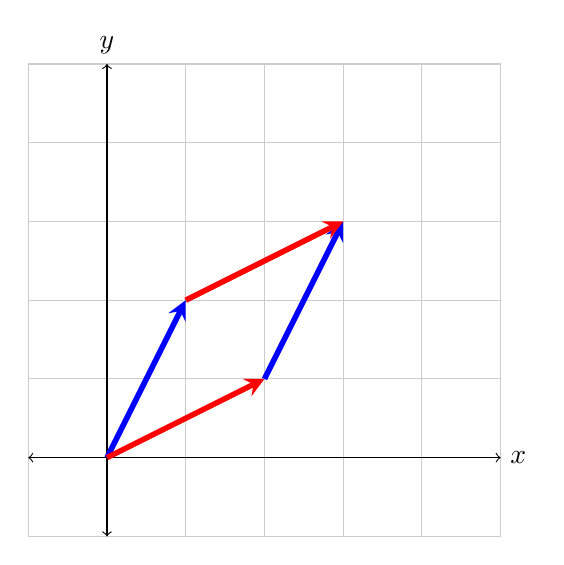
\begin{tikzpicture}
        \draw[thin,gray!40] (-1,-1) grid (5,5);
        \draw[<->] (-1,0)--(5,0) node[right]{$x$};
        \draw[<->] (0,-1)--(0,5) node[above]{$y$};
        \draw[line width=2pt,blue,-stealth](0,0)--(1,2) node[anchor=east] at (.5,1){$\vecu$};
        \draw[line width=2pt, red, -stealth](0,0)--(2,1) node[anchor=north] at (1,.5){$\vecv$};
        \draw[line width=2pt,blue,-stealth](2,1)--(3,3) node[anchor=east] at (.5,1){};
        \draw[line width=2pt, red, -stealth](1,2)--(3,3) node[anchor=north] at (1,.5){};
        \end{tikzpicture}
        \end{center}
        We can then compute the area of this parallelogram by first computing the cross product $\vecu \times \vecv$.  So we have
        \begin{align*}
        \vecu \times \vecv &= (\xhat + 2\yhat)\times(2\xhat + \yhat)\\
        &= 2\xhat \times \xhat + \xhat \times \yhat + 4 \yhat \times \xhat + 2\yhat \times \yhat \\
        &= \zerovec + \zhat - 4\zhat + \zerovec\\
        &= -3\zhat.
        \end{align*}
        Then we have that the area of the parallelogram is
        \[
        \boxed{A = \|\vecu \times \vecv\| = \|-3 \zhat\| = 3.}
        \]
        \end{ex}
        
        \begin{exercise}
        Compute the area of the parallelogram defined by $\vecu=3\xhat + \yhat -\zhat$ and $\vecv=\xhat + 2\yhat -3\zhat$.
        \end{exercise}
        
        %left off editing here...
        %%%%%%%%%%%%%%%%%%%%%%%%%%%%%%%%
        
        \begin{ex}{Angular Velocity and Right-Hand Rule}{angular_velocity}
        For a particle moving along a circle with radius $r$ we can define a quantity called the \emph{angular velocity} and denote it by $\boldsymbol{\vec{\omega}}$.  Then, for example, the time it takes for the particle to travel around the whole circle (the \emph{period}) is
        \[
        \tau = \frac{2\pi r}{\|\boldsymbol{\vec{\omega}}\|}.
        \]
        It turns out that the angular velocity of this particle at any point is given by
        \[
        \boldsymbol{\vec{\omega}}=\frac{\vecr\times \vecv}{\|\boldsymbol{\vec{r}}\|^2}.
        \]
        We can also find $\vecv$ from $\boldsymbol{\vec{\omega}}$ and $\vecr$. Take a look at the figure below and note the orientation of $\boldsymbol{\vec{\omega}}$ relative to the direction the particle travels around the circle.
        \begin{center}
        \begin{figure}[H]
            \centering
            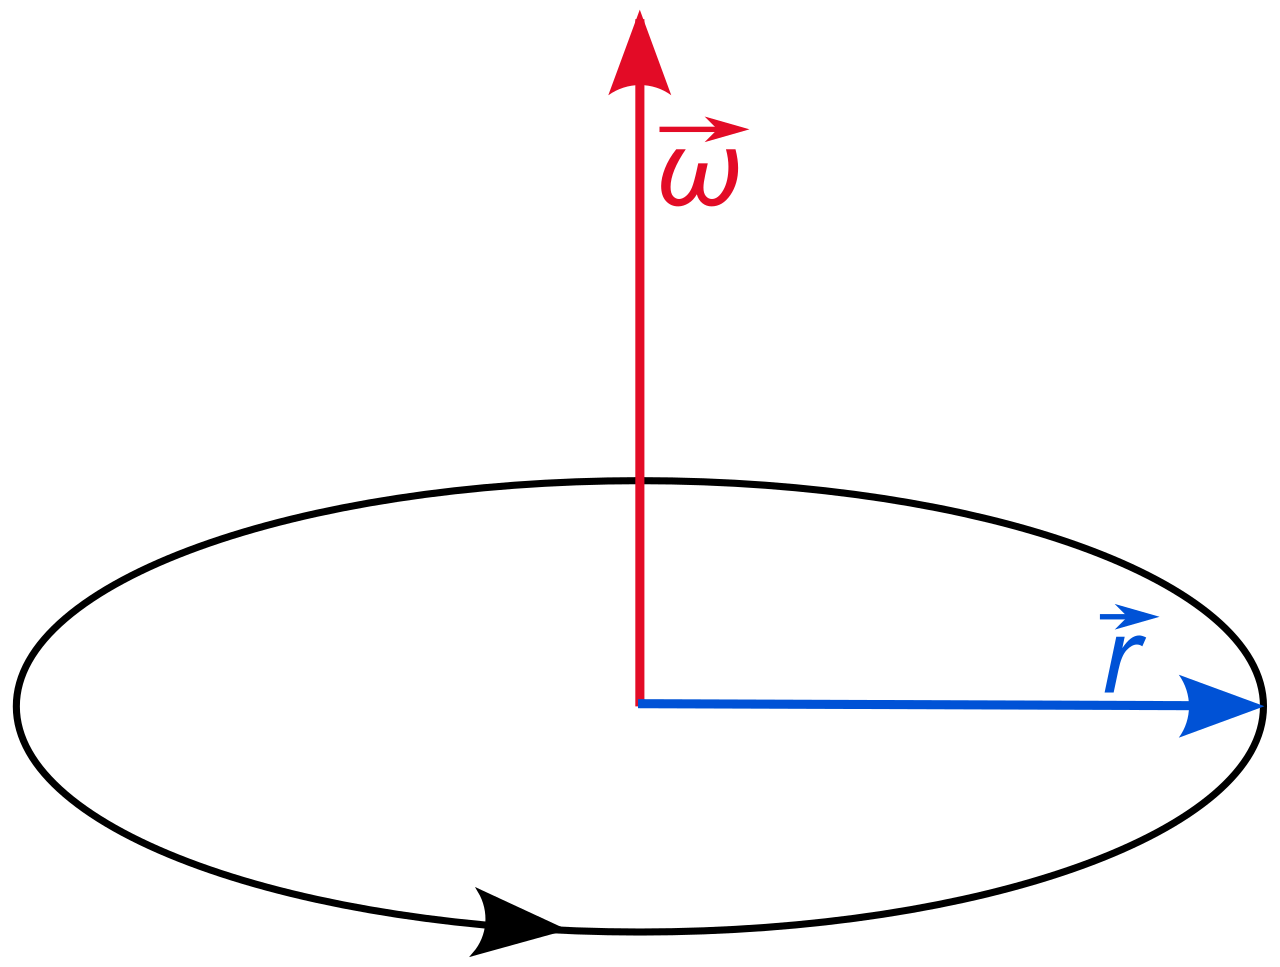
\includegraphics[width=.3\textwidth,bb=0 0 30 30]{Figures/Angular_velocity.png}
            \caption{A particle moving around a circle of radius $\|\vecr\|$ in a counter-clockwise motion.}
            \label{angular-momentum}
        \end{figure}
        \end{center}
        Note that $\vecv$ would be tangent to this circle at the point $\vecr$ and pointing along the direction of travel.
        
        It turns out that $\boldsymbol{\vec{\omega}}$ is a vector pointing perpendicularly to the plane that the circle the particle traverses is in. Which way does $\boldsymbol{\vec{\omega}}$ point? We need the \emph{right-hand rule}!
        \begin{center}
        \begin{figure}[H]
            \centering
            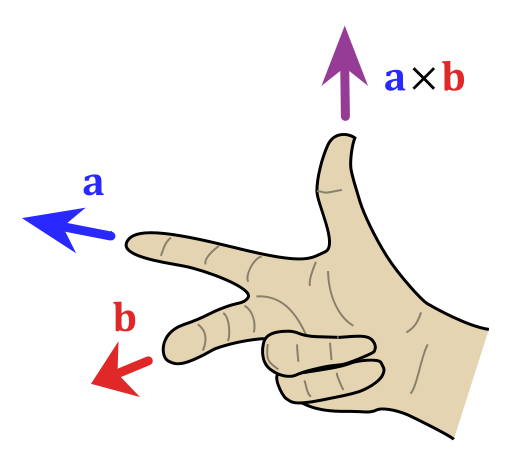
\includegraphics[width=.3\textwidth,bb=0 0 30 30]{Figures/507px-Right_hand_rule_cross_product.png}
            \caption{The right-hand rule.}
        \end{figure}
        \end{center}
        To see how this works, we let $\boldsymbol{\vec{a}}=\vecr$ be our index finger, then $\boldsymbol{\vec{b}}=\vecv$ be our middle finger.  The resulting direction of $\vecr\times \vecv=\boldsymbol{\vec{\omega}}$ is then pointing in the direction we see from Figure \ref{angular-momentum}.
        \end{ex}
        
        
  
        
